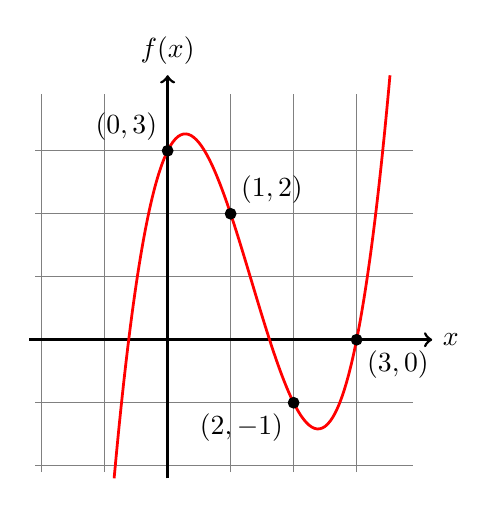
\begin{tikzpicture}[scale=0.8,line width=1pt]
\def\funcpoly{3+2*\x-4*\x*\x+\x*\x*\x}
\draw[very thin,color=gray] (-2.1,-2.1) grid (3.9,3.9);
\draw[->] (-2.2,0) -- (4.2,0) node[right] {$x$};
\draw[->] (0,-2.2) -- (0,4.2) node[above] {$f(x)$};
\draw[color=red,smooth,every node/.style={color=black},mark=*,mark size=2pt,mark options={color=black}]
    plot[domain=-0.84962:0,mark=] (\x,\funcpoly)
    node[above left] {$(0,3)$}
    plot[domain=0:1,mark indices=1] (\x,\funcpoly)
    node[above right] {$(1,2)$}
    plot[domain=1:2,mark indices=1] (\x,\funcpoly)
    node[below left] {$(2,-1)$}
    plot[domain=2:3,mark indices=1] (\x,\funcpoly)
    node[below right] {$(3,0)$}
    plot[domain=3:3.5297,mark indices=1] (\x,\funcpoly)
    ;
\end{tikzpicture}